% ============================================================================
%  DEPTH: Calibrated, Human-Approved Detection of Derelict Fishing Gear
%         in Side-Scan Sonar
%  Two-column research-paper layout (CVPR-like). Compile with:
%      pdflatex DEPTH_paper.tex   (run twice for references)
%  or upload this folder (DEPTH_paper.tex + figures/) to Overleaf.
% ============================================================================
\documentclass[10pt,twocolumn,letterpaper]{article}

\usepackage[letterpaper,top=1in,bottom=1in,left=0.75in,right=0.75in,columnsep=0.3125in]{geometry}
\usepackage{times}
\usepackage[T1]{fontenc}
\usepackage[utf8]{inputenc}
\usepackage{amsmath,amssymb}
\usepackage{graphicx}
\usepackage{booktabs}
\usepackage{multirow}
\usepackage{xcolor}
\usepackage{tikz}
\usetikzlibrary{arrows.meta,positioning,calc,fit,backgrounds,patterns}
\usepackage[font=small,labelfont=bf,skip=4pt]{caption}
\usepackage{enumitem}
\usepackage{microtype}
\usepackage[colorlinks=true,linkcolor=red!60!black,citecolor=green!45!black,urlcolor=magenta!70!black]{hyperref}

\setlist{nosep,leftmargin=*}
\raggedbottom
\setlength{\textfloatsep}{8pt plus 2pt minus 2pt}
\setlength{\floatsep}{6pt plus 2pt minus 2pt}
\setlength{\intextsep}{6pt plus 2pt minus 2pt}
\setlength{\dbltextfloatsep}{8pt plus 2pt minus 2pt}

% Section style close to CVPR
\makeatletter
\renewcommand\section{\@startsection{section}{1}{\z@}{-2.0ex plus -0.5ex minus -.2ex}{1.0ex plus .2ex}{\large\bfseries}}
\renewcommand\subsection{\@startsection{subsection}{2}{\z@}{-1.6ex plus -0.5ex minus -.2ex}{0.6ex plus .2ex}{\normalsize\bfseries}}
\makeatother

\newcommand{\depth}{\textsc{Depth}}
\newcommand{\etal}{et~al.\@}
\newcommand{\eg}{e.g.,}

\title{\Large\bfseries DEPTH: Calibrated, Human-Approved Detection of\\ Derelict Fishing Gear in Side-Scan Sonar}
\author{
  Madhesh\\
  {\normalsize Team Syndicate}\\
  {\small OpenCV AI Competition 2026 \,---\, Agentic Vision \& Best Use of COOL}\\
  {\small\color{magenta!70!black}\url{https://github.com/madhesh60/depth}}
}
\date{}

\begin{document}
\maketitle

% ---------------------------------------------------------------- Abstract --
\begin{abstract}
\itshape
We present \depth{}, a system that turns side-scan sonar surveys into
human-approved cleanup plans for derelict fishing gear (``ghost gear'') and
wreck debris. Prior work treats the problem as object detection and reports an
average score. Instead, we wrap an imperfect detector in an agent that makes a
statistically checkable promise about coverage: with 95\% confidence, at
least 78\% of crab pots reach a human reviewer with one look, and at least
84\% when the agent looks harder. Both promises are fitted on held-out
recordings and verified once on unseen recordings, where they held at
81.1\% and 86.0\%. The agent also tests whether its promise applies to the
recording at hand; it withdrew the promise in 22 of 22 surveys from a different
sonar. Measured sonar geometry places each finding on the map, and without it
95 of 142 positions fall outside their own error circle. The whole pipeline runs
on a CPU with OpenCV~5 at 138.5\,ms per frame on AWS Graviton4. The detector
itself is modest (crab-pot AP@0.5 of 0.482, F1 of 0.41 against 0.71--0.73 for the
state of the art), and we report this openly: our contribution is the layer that
makes such a detector dependable.
\end{abstract}

% ------------------------------------------------------------ Introduction --
\section{Introduction}

Fishing gear that is lost at sea keeps catching animals. An estimated
640{,}000 tonnes of gear is lost every year~\cite{fao}. A lost crab pot is a
baited cage; animals that enter it die and become bait for the next.
% ---------------------------------------------------------------- Figure 1 --
\begin{figure}[t]
\centering
\resizebox{\columnwidth}{!}{%
\begin{tikzpicture}[
  stage/.style={draw=black!70,rounded corners=1.5pt,fill=black!3,minimum width=2.35cm,minimum height=0.42cm,font=\footnotesize,inner sep=1.5pt},
  arr/.style={-{Stealth[length=4pt]},thick,black!70}]
  \node[inner sep=0] (in) {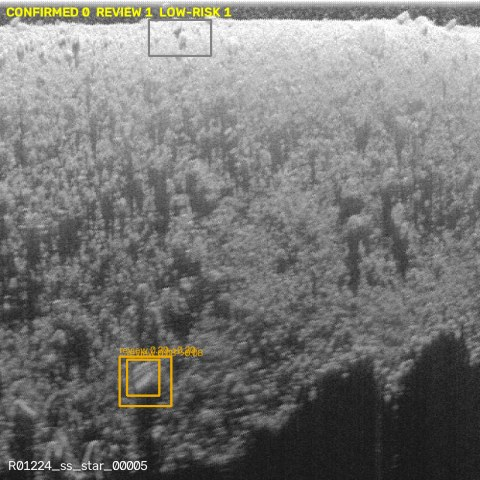
\includegraphics[width=2.35cm]{figures/sonar_frame.png}};
  \node[below=1pt of in,font=\scriptsize,align=center] {side-scan frame};
  \node[stage,right=0.3cm of in,yshift=1.05cm] (s1) {1. Canonicalise};
  \node[stage,below=0.07cm of s1] (s2) {2. See (\texttt{cv2.dnn})};
  \node[stage,below=0.07cm of s2] (s3) {3. Prove};
  \node[stage,below=0.07cm of s3] (s4) {4. Decide ($\geq$78\,\%)};
  \node[stage,below=0.07cm of s4] (s5) {5. Act};
  \node[inner sep=0,draw=black!30,right=0.3cm of s3] (out) {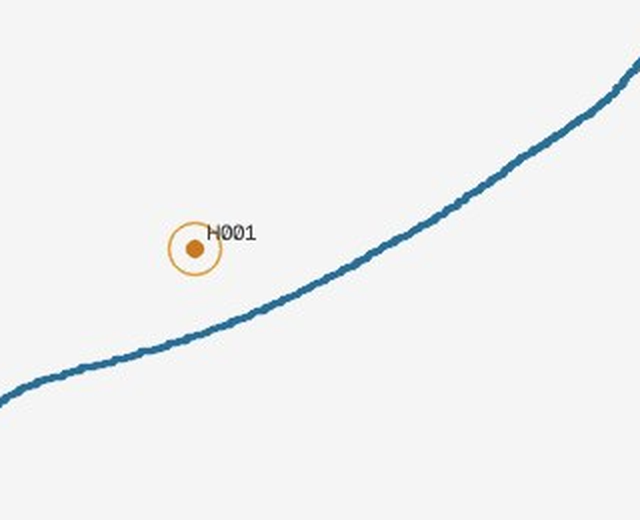
\includegraphics[width=2.35cm]{figures/gps_map.png}};
  \node[below=1pt of out,font=\scriptsize,align=center] {plan for approval};
  \draw[arr] (in.east) -- (in.east -| s3.west);
  \draw[arr] (s3.east) -- (out.west);
  \node[draw=black!40,dashed,rounded corners,fit=(s1)(s5),inner sep=2.5pt,label={[font=\scriptsize]above:agent core loop}] {};
\end{tikzpicture}}
\caption{\textbf{The \depth{} system.} A side-scan frame passes through five
OpenCV~5 stages run by a goal-driven agent. The agent (1)~measures the sonar
geometry, (2)~detects candidates with a YOLO11 network in \texttt{cv2.dnn},
(3)~attaches physical evidence, (4)~sends every candidate above a calibrated
threshold to a person, and (5)~turns the findings into a georeferenced plan
that a named person must approve.}
\label{fig:teaser}
\end{figure}
 In
Virginia alone, a six-year programme counted more than 31{,}000 animals killed
by derelict blue-crab pots, and removing 43{,}968 pots was estimated to return
38.17 million lb of harvestable crab, worth about \$33.5 million~\cite{vims}.

Derelict gear lies 5--50\,m below the surface, out of reach of optical and
radar satellites~\cite{russwurm2023}. Survey teams therefore use
\emph{side-scan sonar}, which images the seabed acoustically: an object appears
as a bright return followed by a dark acoustic shadow. Each hour of survey
produces a few hundred sonar frames, and today a trained analyst inspects every
one.

Automatic detectors exist~\cite{ghostvision}, but a detector alone does not
answer the questions a cleanup crew must answer. How many pots did it miss on
\emph{this} survey? Does its accuracy hold on \emph{this} sonar? Where exactly
should the boat go? In our experiments, a threshold tuned on one sonar recovered
only 11\% of the pots on another (Sec.~\ref{sec:detector}). A box and a
confidence score are not a plan, and they give no warning when they cannot be
trusted.

We take a different view. Rather than claiming a better detector, \depth{}
builds a decision layer around an imperfect one. Our contributions are:
\begin{itemize}
\item A \textbf{recall guarantee} fitted with Clopper--Pearson bounds and
Learn-Then-Test~\cite{clopper,ltt}, corrected for correlated frames with a block
bootstrap~\cite{kunsch}, and verified once on unseen recordings.
\item An \textbf{applicability test} based on conformal p-values~\cite{vovk}
that withdraws the guarantee on out-of-distribution data.
\item \textbf{Measured sonar geometry} (bottom tracking, slant-to-ground
correction) that changes where the boat is sent.
\item A \textbf{goal-driven agent} that selects the perception mode, re-plans
from its own measurements and requests human approval for every action.
\item A torch-free \textbf{CPU runtime} on OpenCV~5, and an evaluation that
reports per-class results, cross-sensor results and negative results.
\end{itemize}

% ------------------------------------------------------------ Related work --
\section{Related Work}

\textbf{Marine debris from remote sensing.} Rußwurm \etal{}~\cite{russwurm2023}
detect floating debris in Sentinel-2 imagery and attribute their performance to
dataset design rather than model choice. The modality differs from ours, but we
reach the same conclusion for sonar (Sec.~\ref{sec:data}).

\textbf{Detection in side-scan sonar.} GhostVision~\cite{ghostvision} released
the crab-pot dataset we use and reports F1 of 0.71--0.73 on its official split.
PING-Mapper~\cite{pingmapper} provides open tools and recordings for
recreation-grade sonar. These works output detections; none provides coverage
guarantees, applicability checks or survey planning.

\textbf{Real-time detectors.} YOLO~\cite{yolo} frames detection as a single
regression over the whole image. We use its descendant YOLO11~\cite{yolo11},
exported to ONNX~\cite{onnx} and executed in OpenCV~5~\cite{opencv}.

\textbf{Distribution-free guarantees.} Clopper--Pearson intervals~\cite{clopper}
bound a binomial rate; Learn-Then-Test~\cite{ltt} selects thresholds with risk
control; conformal prediction~\cite{vovk} gives finite-sample p-values for
atypicality; the block bootstrap~\cite{kunsch} handles dependent samples. We
combine these to turn a detector's scores into an operational promise.
Table~\ref{tab:compare} summarises how \depth{} differs from current practice.

\begin{table}[t]
\centering\small
\setlength{\tabcolsep}{2.5pt}
\begin{tabular}{@{}lcccc@{}}
\toprule
 & Satellite & Manual & Detector & \depth{} \\
\midrule
Sees 5--50\,m seabed & -- & \checkmark & \checkmark & \checkmark \\
Coverage guarantee & -- & -- & -- & \checkmark \\
Knows when it does not apply & -- & \checkmark & -- & \checkmark \\
Measured sonar geometry & -- & -- & -- & \checkmark \\
One review item per object & -- & \checkmark & -- & \checkmark \\
Routes and re-survey plans & -- & -- & -- & \checkmark \\
Human approval of actions & -- & \checkmark & -- & \checkmark \\
Analyst effort per survey-hour & -- & high & -- & reduced$^\dagger$ \\
\bottomrule
\end{tabular}
\caption{\textbf{Comparison with current practice.} Satellite: optical and
radar debris mapping~\cite{russwurm2023}. Manual: analyst review of every frame.
Detector: a sonar detector used on its own~\cite{ghostvision}.
$^\dagger$Under assumed timings (Sec.~\ref{sec:effort}).}
\label{tab:compare}
\end{table}

% ------------------------------------------------------------------ Method --
\section{The \depth{} System}
\label{sec:method}

\begin{figure*}[t]
\centering
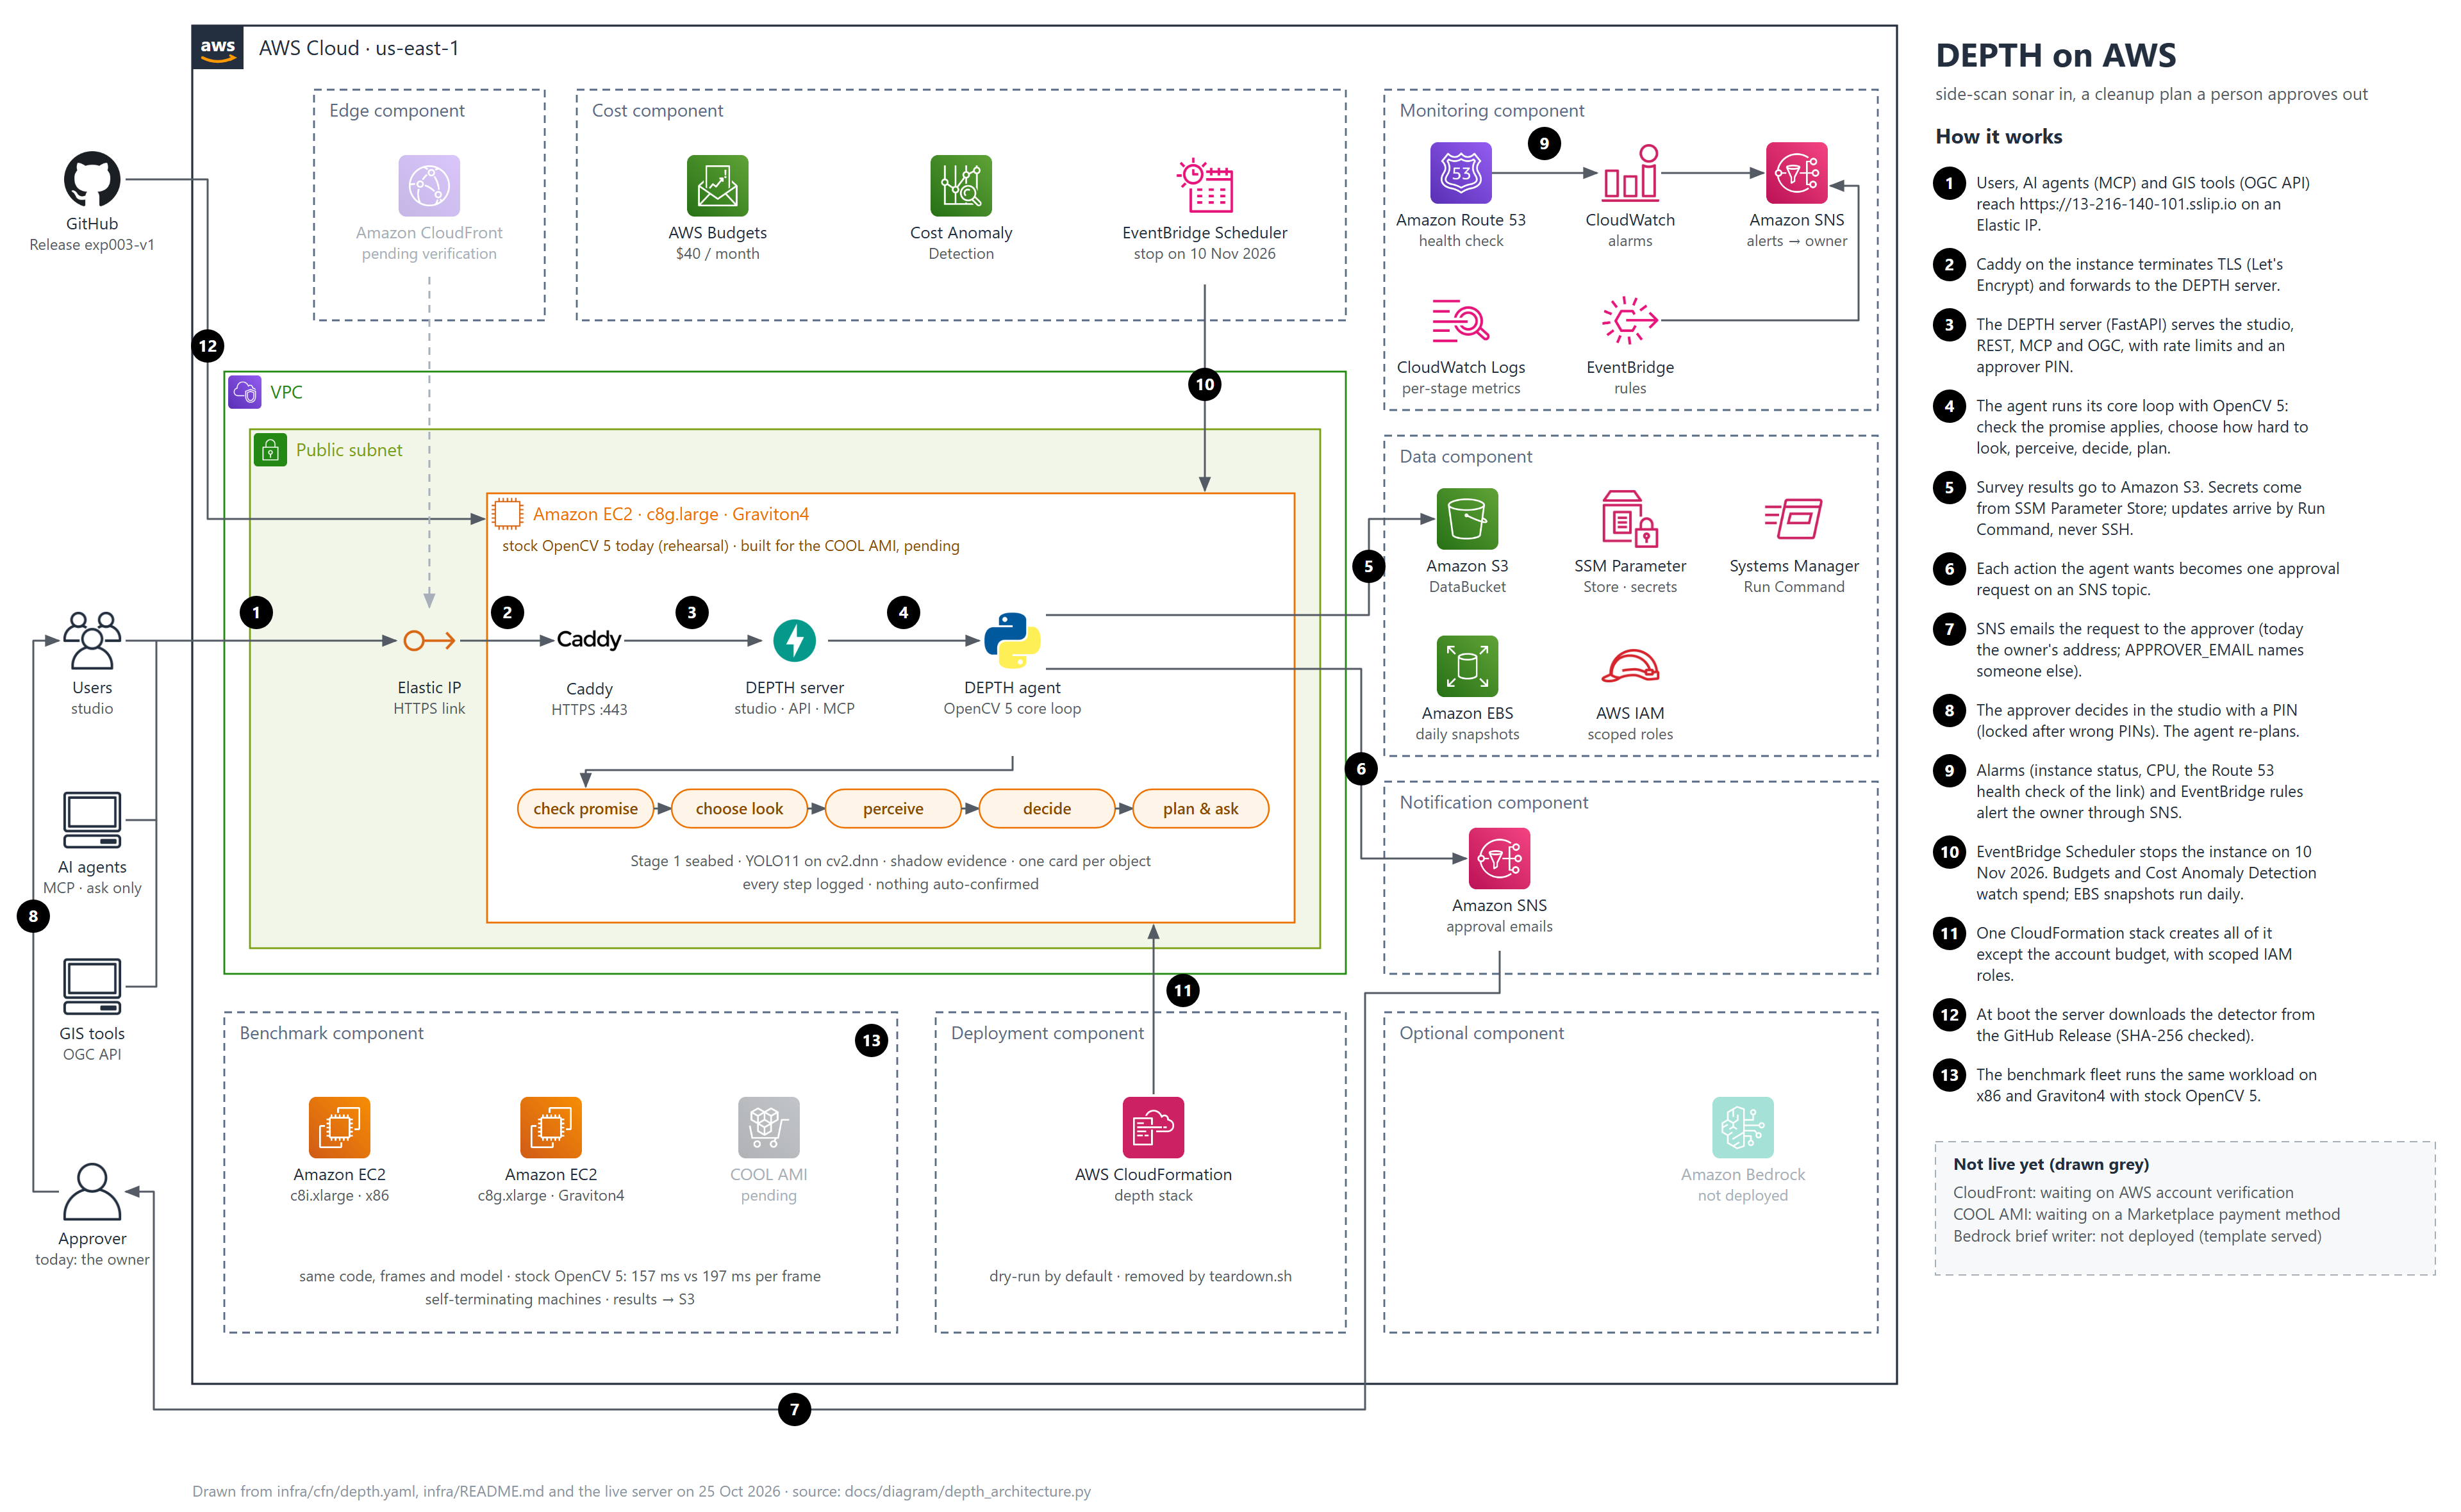
\includegraphics[width=\textwidth]{figures/depth_architecture.png}
\caption{\textbf{\depth{} on AWS, as deployed.} Users, AI agents (MCP) and GIS
tools (OGC API) reach an EC2 Graviton4 instance through an Elastic IP and Caddy
(1--3). On the instance, the agent runs its core loop on OpenCV~5: check that
the promise applies, choose the look, perceive, decide, plan and ask (4).
Results go to S3 and secrets come from SSM (5). Each action the agent wants
becomes an approval request emailed through SNS, and a named person decides in
the studio with a PIN (6--8). CloudWatch, Route~53 and EventBridge alert the
owner (9--10); one CloudFormation stack creates the deployment (11); the detector
is fetched from a SHA-256-checked GitHub release (12); a benchmark fleet compares
x86 and Graviton4 (13). Grey components are not live yet.}
\label{fig:arch}
\end{figure*}

\subsection{Agent Loop}
Each survey is run by an agent toward an operator goal: a recall level plus
budgets for compute, analyst and boat time (Fig.~\ref{fig:arch}). The agent
(i)~discards unusable frames and logs them as incidents; (ii)~tests whether its
promise applies (Sec.~\ref{sec:applic}); (iii)~selects the cheapest calibrated
perception mode that meets the goal within the compute budget; (iv)~perceives
every frame while measuring its own pace, and falls back to the standard mode if
the budget would be exceeded; and (v)~plans and files one approval request per
action. Each decision and the options it considered are written to a replayable
log. A request that cannot be met (\eg{} 95\% recall, above the detector's
ceiling) is refused with the strongest promise the agent can keep.

\subsection{Sonar Canonicalisation}
\label{sec:stage1}
Stage~1 measures geometry; it does not filter detections. It converts palettes
to luminance and sets orientation from a source rule (an automatic guess was
correct on only 26\% of frames). For each ping it tracks the first
water-to-seabed transition to obtain the sonar altitude $a$, then smooths it
along track. With slant range $s$, the ground range is
\begin{equation}
g=\sqrt{s^{2}-a^{2}},
\end{equation}
which Stage~1 applies to the whole frame with \texttt{cv2.remap}
(Fig.~\ref{fig:geom}). It also masks the water column, where no seabed object
can appear. For raw recordings the range scale is measured as sonar depth over
tracked altitude, giving $2.03$\,cm per sample $\pm10.2\%$, and the track is
cross-checked against the depth sounder every 500 pings.

Bottom tracking is validated without labels. Port and starboard channels share
one transducer, so their altitudes must agree. On 107 single-copy frames they
agree to a median of 1.6\,px, compared with 5.3\,px for random pairs; 97\% of
frames were tracked and the remainder were marked \emph{not measured}. Stage~1
takes about 5\,ms per $640\times640$ frame.

\begin{figure}[t]
\centering
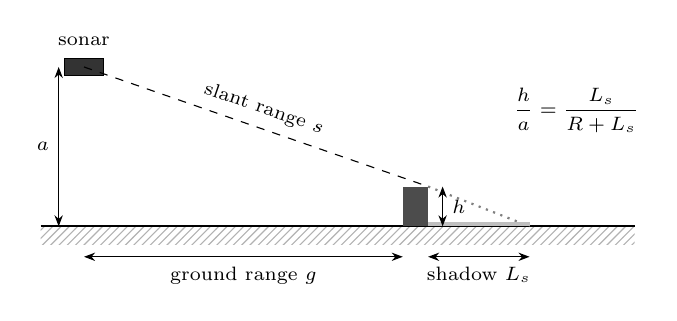
\begin{tikzpicture}[scale=0.92,>={Stealth[length=4pt]},font=\scriptsize]
  \fill[pattern=north east lines,pattern color=black!30] (0,0) rectangle (8.2,-0.25);
  \draw[thick] (0,0) -- (8.2,0);
  \node[draw,fill=black!80,minimum width=0.5cm,minimum height=0.22cm,inner sep=0] (sonar) at (0.6,2.2) {};
  \node[above=1pt of sonar] {sonar};
  \draw[<->] (0.25,0) -- node[left] {$a$} (0.25,2.2);
  \fill[black!70] (5.0,0) rectangle (5.35,0.55);
  \draw[dashed] (0.6,2.2) -- (5.35,0.55);
  \draw[black!50,dotted,thick] (5.35,0.55) -- (6.75,0);
  \node[above,rotate=-19] at (3.0,1.38) {slant range $s$};
  \fill[black!25] (5.35,0) rectangle (6.75,0.06);
  \draw[<->] (5.35,-0.42) -- node[below] {shadow $L_s$} (6.75,-0.42);
  \draw[<->] (0.6,-0.42) -- node[below] {ground range $g$} (5.0,-0.42);
  \draw[<->] (5.55,0) -- node[right] {$h$} (5.55,0.55);
  \node[font=\scriptsize\itshape] at (7.4,1.6) {$\dfrac{h}{a}=\dfrac{L_s}{R+L_s}$};
\end{tikzpicture}
\caption{\textbf{Sonar geometry.} Stage~1 tracks the altitude $a$ and converts
slant range to ground range. The acoustic shadow behind an object gives its
height relative to the altitude by similar triangles ($R$: range to the object).}
\label{fig:geom}
\end{figure}

\subsection{Detection}
The detector is YOLO11s~\cite{yolo11} with two classes, \texttt{ghost\_gear} and
\texttt{wreck\_debris}. It is trained in PyTorch, exported to ONNX and executed
by \texttt{cv2.dnn}, so the server has no PyTorch dependency. Frames are
letterboxed to $640\times640$; the network outputs 8{,}400 candidates, which are
reduced by class-aware non-maximum suppression at IoU 0.45. OpenCV~5 provides two
inference engines that produce identical outputs here (634 of 634 detections);
the server times both at start-up and keeps the faster one, which on Graviton4 is
the classic engine at 1.41--1.47$\times$ the speed of the default. Every class
name and threshold is read from a per-model calibration file.

\subsection{Physical Evidence}
For each candidate, \depth{} reports (i)~whether the box lies above the tracked
seabed; (ii)~the contrast of its thin-line acoustic shadow against same-size
flank windows (CLEAR, WEAK or NONE); and (iii)~its relative height
$h/a=L_s/(R+L_s)$, given in metres only when the altitude is measured in
metres. Evidence is shown to the reviewer but never removes a candidate: used as
a filter, the shadow reduced precision from 0.59 to 0.31--0.50, and it separates
true from false detections only weakly (AUC 0.563).

\subsection{Calibrated Recall Guarantee}
\label{sec:guarantee}
Candidates above a review threshold $\tau$ go to a person; the rest are kept for
audit. We choose $\tau$ on a \emph{calibration} split of three whole recordings
(163 frames, 186 pots) that the detector never saw. A pot is \emph{reached} if a
box at score $\geq\tau$ overlaps it with IoU $\geq0.3$; a pot never proposed
counts as a miss. If $k$ of $n$ pots are reached, the one-sided 95\% lower bound
on recall is
\begin{equation}
\underline{r}(\tau)=\mathrm{Beta}^{-1}\!\left(0.05;\,k,\,n-k+1\right).
\end{equation}
Thresholds are tested in a fixed order from strict to loose
(Learn-Then-Test~\cite{ltt}). A requested 90\% recall is infeasible because the
detector proposes only 85\% of pots at its lowest score (its \emph{recall
ceiling}), so the agent promises the best supportable bound. At $\tau=0.060$,
157 of 186 pots are reached (84.4\%), giving $\underline{r}=79.4\%$.

\textbf{Correlated frames.} Clopper--Pearson assumes independent pots, but
neighbouring frames and the two channels of one ping image the same seabed. We
resample blocks of 8 consecutive ping indices within each recording (20{,}000
replicates~\cite{kunsch}). The bound falls to 78.2\%, a design effect of 1.86
(186 pots carry the information of about 100 independent ones). By a rule
registered before computation, the promise is restated to \textbf{$\geq$78\%}.

\textbf{Looking harder.} A second mode adds a $2\times2$ tile pass (tile side 60\%
of the frame, the training scale), merging boxes at IoU $\geq0.5$. It raises the
recall ceiling from 0.850 to 0.892 (paired bootstrap $+0.043$, 95\% CI
$[+0.016,+0.076]$) and supports \textbf{$\geq$84\%} at $\tau=0.055$, at the cost
of five network passes per frame instead of one.

\textbf{One card per object.} Two boxes of the same class in one frame share one
review card when $\mathrm{area}(A\cap B)/\min(\mathrm{area}(A),\mathrm{area}(B))
\geq0.5$. No box is discarded, so the set of reached pots is unchanged. A
calibrated probability $P(\mathrm{pot})$ orders the queue, and its sum forecasts
the yield of an analyst's time budget.

No precision guarantee is achievable (best bound 0.565 against a 0.85 target),
so nothing is confirmed automatically.

\subsection{Applicability Test}
\label{sec:applic}
A promise fitted on one sonar should not be applied to another. For each frame we
compute eight OpenCV statistics: brightness, contrast, Laplacian texture, Sobel
along/across-track anisotropy, dark and saturated pixel shares, HSV saturation
and histogram distance to the calibration recordings. These yield a strangeness
score $s$ and a conformal p-value against the $n=163$ calibration frames,
\begin{equation}
p=\frac{1+\left|\{j:s_j\geq s_{\mathrm{new}}\}\right|}{n+1}.
\end{equation}
A frame is atypical if $p\leq0.05$. The promise is withdrawn when the 95\% lower
bound of a survey's atypical share exceeds 0.20, a limit fixed on training
recordings. The agent then takes the cheapest look and requests a full manual
review.

\subsection{Planning and Human Approval}
Findings are geotagged from the GPS fix and heading of their own ping at the
Stage-1 ground range, with error radius
$r=3\,\mathrm{m}+R\,(u_{\mathrm{scale}}+\sin6^{\circ})$; without GPS no
coordinates are produced. Objects split across frames are stitched, and repeat
sightings are merged. The planner builds inspection and recovery routes and
opposite-side re-survey passes, ranked by expected information
$\sum p(1-p)$ per boat-minute. Outputs are exported as GeoJSON, GPX, KML, CSV and
JSON with a provenance stamp. Every action requires approval by a named person
with a PIN; external AI agents connected through MCP can request but never
approve.

% -------------------------------------------------------------------- Data --
\section{Data and Training}
\label{sec:data}

\textbf{Sources.} Crab-pot frames come from the GhostVision dataset~\cite{ghostvision};
wreck frames from SeabedObjects-KLSG and AI4Shipwrecks; empty seabed from
Marine PULSE. Two raw Humminbird recordings with per-ping GPS from
PING-Mapper~\cite{pingmapper} (150.6\,s and 1\,h, no labels) are used only for
geometry and false-alarm load.

\textbf{Evaluation traps.} The released archive contains baked-in augmentation:
1{,}615 frames appear as 5{,}275 near-copies, and the official 398 test images
are 214 unique frames. We therefore score \emph{unique frames} only, split by
recording rather than by frame, and moved a validation split that came from a
different sonar into a separate cross-sonar test. Table~\ref{tab:splits}
summarises the splits.

\begin{table}[t]
\centering\small
\setlength{\tabcolsep}{3pt}
\begin{tabular}{@{}llr@{}}
\toprule
Split & Content & Size \\
\midrule
v2b train & side-scan, 2 classes & 1{,}773 frames \\
v2b train (tiled) & full frames + $2\times2$ tiles & 4{,}839 images \\
Calibration & Rec10/12/16, held out whole & 163 fr. / 186 pots \\
Verification & Rec8/9/14, scored once & 199 fr. / 264 pots \\
v2b test & crab pot + wreck & 285 frames \\
Official-398 & GhostVision split & 398 img. / 567 pots \\
Cross-sonar & another sonar & 555 img. / 1{,}265 pots \\
\bottomrule
\end{tabular}
\caption{\textbf{Data splits.} All counts are unique frames. The calibration
and verification splits are the recording-level subsets used for the guarantee.}
\label{tab:splits}
\end{table}

\textbf{Training.} YOLO11s is initialised from COCO weights and trained at
640\,px on full frames plus $2\times2$ tiles, with cut boxes inpainted so that no
tile shows an unlabelled partial object. We use SGD (learning rate 0.01, batch
64, seed 42) for up to 150 epochs with early stopping (104 epochs, 135\,min on a
T4). Augmentation respects sonar physics: horizontal flips (along-track) are
allowed; vertical flips, rotations and hue shifts are not, because they produce
physically impossible sonograms. The checkpoint is selected by crab-pot AP@0.5 on
the calibration recordings. An earlier run with the framework's automatic
optimiser silently selected AdamW at a learning rate of 0.00167 and underfit;
every subsequent run sets the optimiser explicitly.

\begin{table}[t]
\centering\small
\setlength{\tabcolsep}{4pt}
\begin{tabular}{@{}llc@{}}
\toprule
Run & Change & Val. AP@0.5 \\
\midrule
EXP-002 / 002s & 1024 / 640\,px, auto optimiser & 0.26 / 0.29 \\
\textbf{EXP-003} & \textbf{explicit SGD, fixed tiles} & \textbf{0.39} \\
EXP-003f & full frames, 300 epochs & 0.36 \\
EXP-004 / 004g & cleaned data / one class & 0.365 / $-$0.07 \\
EXP-005 / 005a & cleaned data + jitter & 0.292 / 0.327 \\
\bottomrule
\end{tabular}
\caption{\textbf{Model selection} on the calibration recordings (crab-pot AP@0.5
through \texttt{cv2.dnn}). EXP-003 is deployed; five follow-up runs did not
improve on it.}
\label{tab:runs}
\end{table}

The remaining gap is in the data. Of 459 training frames with wreck labels, 389
are screenshots of consumer fish-finders rather than side-scan sonar, and
45--57\% of side-scan wreck boxes extend past the frame edge
(Table~\ref{tab:runs}).

% ------------------------------------------------------------- Experiments --
\section{Experiments}

\textbf{Protocol.} Thresholds are tuned on calibration data; each test split is
scored once; only unique frames count; every number names its split. AP@0.5
uses VOC all-point interpolation~\cite{voc} and AP@0.5:0.95 follows
COCO~\cite{coco}; confidence intervals use 1{,}000 bootstrap resamples. All
results use the deployed ONNX model in \texttt{cv2.dnn}.

\subsection{Detector Accuracy}
\label{sec:detector}

\begin{table}[t]
\centering\small
\setlength{\tabcolsep}{3.5pt}
\begin{tabular}{@{}lccc@{}}
\toprule
Metric & Crab pot & Wreck & Split \\
\midrule
AP@0.5 & \textbf{0.482} & 0.156 & v2b test \\
\quad 95\% CI & 0.43--0.55 & 0.10--0.25 & \\
AP@0.5:0.95 & 0.165 & 0.047 & v2b test \\
P / R / F1 (val. thr.) & .50 / .47 / .49 & .35 / .11 / .17 & v2b test \\
mAP@0.5 (2 classes) & \multicolumn{2}{c}{0.319} & v2b test \\
\midrule
F1 / AP@0.5 & 0.41 / 0.39 & -- & Official-398 \\
\quad GhostVision~\cite{ghostvision} & F1 0.71--0.73 & -- & Official-398 \\
AP@0.5 / recall & 0.34 / 0.11 & -- & Cross-sonar \\
\bottomrule
\end{tabular}
\caption{\textbf{Detector accuracy} of EXP-003. Thresholds were tuned on
validation. The cross-sonar row shows that the threshold does not transfer
between sensors.}
\label{tab:detector}
\end{table}

Table~\ref{tab:detector} and Fig.~\ref{fig:pr} report detector accuracy.
Crab-pot AP@0.5 is 0.482 on unique test frames; the wreck class is weak.
On the official GhostVision split our F1 is 0.41 against their reported
0.71--0.73, a real gap that we do not claim to close. On a different sonar,
AP@0.5 is 0.34 but recall at the validation threshold is only 0.11: scores, and
therefore thresholds, do not transfer between sensors. This motivates both the
calibrated threshold and the applicability test.

\begin{figure}[t]
\centering
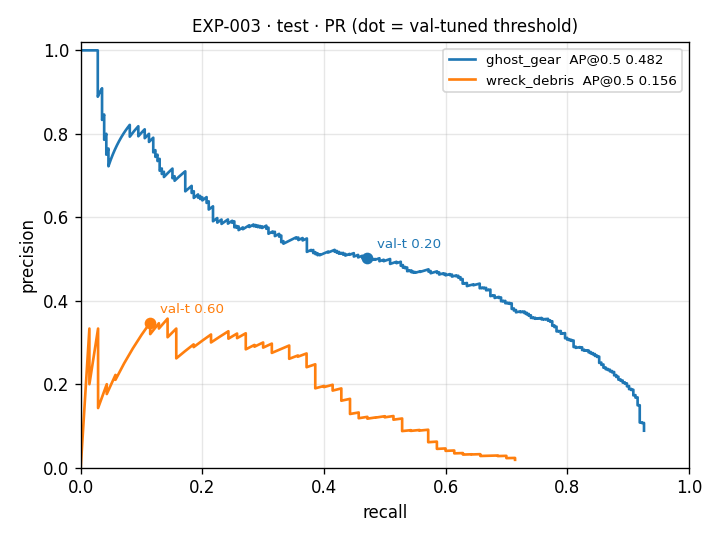
\includegraphics[width=0.92\columnwidth]{figures/pr_exp003_test.png}
\caption{\textbf{Precision--recall curves} of EXP-003 on v2b test. Dots mark the
validation-tuned operating points.}
\label{fig:pr}
\end{figure}

\subsection{Recall Guarantee}

\begin{table}[t]
\centering\small
\setlength{\tabcolsep}{2.6pt}
\begin{tabular}{@{}lcccccc@{}}
\toprule
Mode & Passes & $\tau$ & Cal.\ recall & Promise & Ver.\ recall & Held \\
\midrule
Standard & 1 & 0.060 & 84.4\% & $\geq$78\% & \textbf{81.1\%} (76.7) & \checkmark \\
Look harder & 5 & 0.055 & 88.7\% & $\geq$84\% & \textbf{86.0\%} (82.0) & \checkmark \\
\bottomrule
\end{tabular}
\caption{\textbf{Recall guarantee.} Fitted on the calibration recordings
(186 pots) and verified once on the verification recordings (264 pots).
Parentheses give the 95\% lower bound on verification.}
\label{tab:promise}
\end{table}

Both promises held on unseen recordings (Table~\ref{tab:promise}). For
comparison, the earlier four-class model EXP-001 supported only $\geq$63\% with
the same code, so a better detector translates directly into a stronger promise.
Six re-scoring policies (re-looking at each candidate with zoom or CLAHE) did not
improve ranking over raw confidence (best AUC gain $+0.005$, 95\% CI
$[-0.002,+0.012]$), so no compute is spent on them.

The promise is a pooled rate over recordings, not a per-survey guarantee.
Figure~\ref{fig:perrec} shows recall per recording: the standard promise is met
on 5 of 6 recordings, and the largest test recording (Rec9, 162 pots) reaches
74.7\%. In leave-one-recording-out refits on the calibration split, the standard
promise held in 3 of 3 cases and the look-harder promise in 2 of 3.

\begin{figure}[t]
\centering
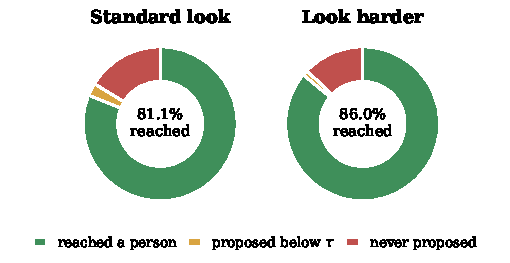
\includegraphics[width=\columnwidth]{figures/pot_outcomes.pdf}
\caption{\textbf{Error analysis} of the 264 verification pots. Misses are
dominated by pots the detector never proposes at any score (its recall ceiling),
not by the choice of threshold.}
\label{fig:outcomes}
\end{figure}

\textbf{Error analysis.} Figure~\ref{fig:outcomes} breaks down where each of the
264 verification pots ends up. With one look, 43 pots (16.3\%) are never
proposed at any score and only 7 are proposed below the threshold; looking
harder recovers 9 of the never-proposed pots. Raising recall further therefore
requires a better detector, not a different threshold.

\begin{figure}[t]
\centering
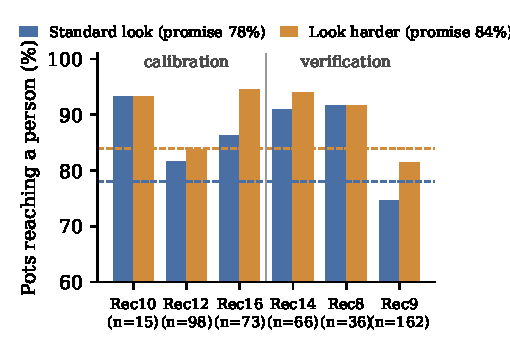
\includegraphics[width=\columnwidth]{figures/per_recording.pdf}
\caption{\textbf{Recall per recording} at each mode's fixed threshold. Dashed
lines mark the promises. The guarantee holds for the pooled rate; individual
recordings vary.}
\label{fig:perrec}
\end{figure}

\subsection{Applicability, Card Grouping and Geometry}

\textbf{Applicability.} The test kept the promise on all three verification
recordings and withdrew it in 22 of 22 cross-sonar surveys, where one look
reaches only 23.9\% of pots against the promised 78\%. It also withdrew the
promise on both raw river recordings, which come from a different sonar.

\textbf{One card per object.} On the verification split, grouping reduces review
cards per frame from 2.68 to 1.81 ($-$33\%) in the standard mode and from 3.86 to
2.32 ($-$40\%) when looking harder. The same 214 and 227 of 264 pots reach a
person, and only 1 of 462 cards holds two labelled pots.

\textbf{Does OpenCV output change decisions?} We re-ran 80 test frames (143
hazards) with Stage-1 geometry withheld and, separately, with shadow evidence
withheld (Table~\ref{tab:causal}). Neither changes tiers or queue order, by
design. Withholding Stage~1, however, moves pins by a median of 9.1\,m and
pushes 95 of 142 outside their own error circle: geometry determines where the
boat is sent.

\begin{table}[t]
\centering\small
\setlength{\tabcolsep}{4pt}
\begin{tabular}{@{}lcc@{}}
\toprule
Downstream decision & w/o Stage 1 & w/o shadow \\
\midrule
Tier changes / Kendall $\tau$ of queue & 0 / 1.0 & 0 / 1.0 \\
Pin shift, median / max & \textbf{9.1 / 15.7\,m} & 0 \\
Pins outside own error circle & \textbf{95 of 142} & 0 \\
Re-survey passes unchanged & 35 of 39 & 39 of 39 \\
\bottomrule
\end{tabular}
\caption{\textbf{Counterfactual trace} on 80 v2b test frames. Stage~1 changes
where the boat goes, not what is reviewed.}
\label{tab:causal}
\end{table}

\subsection{Analyst Effort}
\label{sec:effort}

\begin{figure}[t]
\centering
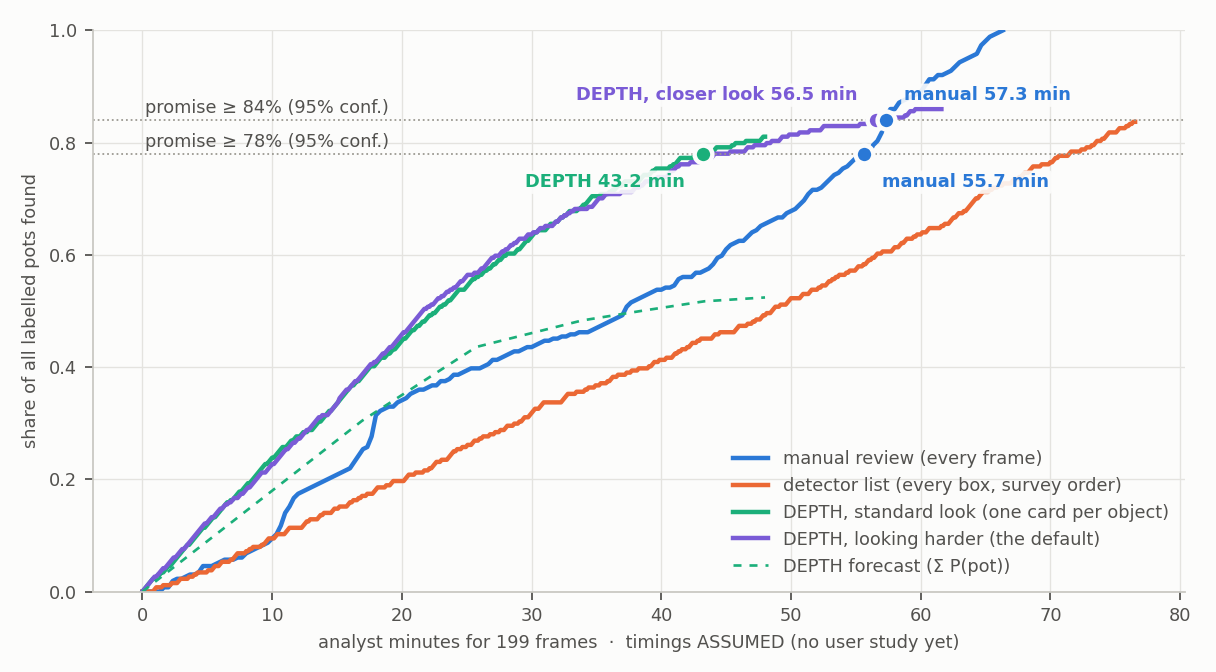
\includegraphics[width=\columnwidth]{figures/effort_curve.png}
\caption{\textbf{Share of pots found against analyst minutes} on the 199
verification frames, assuming 20\,s per frame for manual review and 8\,s per
card. Timings are assumptions until a user study is run.}
\label{fig:effort}
\end{figure}

Figure~\ref{fig:effort} compares manual review of every frame, a list of all
detector boxes, and \depth{}'s queue. Under the assumed timings, \depth{} reaches
its promise in 43.2\,min (standard) and 56.5\,min (look harder), against 55.7 and
57.3\,min for manual review. The break-even time per card, below which \depth{}
is faster, is 10.31\,s and 8.11\,s; it does not depend on the assumed card time.
On empty seabed, which dominates real surveys, \depth{} needs 34 and 47\,min per
survey-hour against 56 for manual review. Before card grouping \depth{} was slower
than manual review in both modes. The queue's $\sum P(\mathrm{pot})$ forecast
underestimates the true yield by 34\% (136.4 forecast, 206 actual).

\subsection{Runtime}

\begin{table}[t]
\centering\small
\setlength{\tabcolsep}{3pt}
\begin{tabular}{@{}llrr@{}}
\toprule
Host (stock OpenCV 5) & Mode & ms/frame & FPS \\
\midrule
c8g.xlarge Graviton4, 4 vCPU & standard & \textbf{138.5} & 7.2 \\
c8i.xlarge x86, 4 vCPU & standard & 145.8 & 6.8 \\
c8g.xlarge / c8i.xlarge & look harder & 655 / 693 & 1.5 / 1.4 \\
c8g.large Graviton4, 2 vCPU & std / harder & 268 / 1{,}300 & 3.7 / 0.8 \\
Graviton4, 1 core & standard & 435 & 2.3 \\
\bottomrule
\end{tabular}
\caption{\textbf{Runtime} (median per frame, full product path). The network
forward pass accounts for 92--99\% of the time.}
\label{tab:speed}
\end{table}

Table~\ref{tab:speed} reports latency on AWS. The standard mode meets the
300\,ms and 5\,FPS targets on 4 vCPUs; looking harder does not, but a side-scan
frame arrives only every 13--21\,s. A one-hour recording was processed end to end
in 46\,s (real-time factor 0.0127) at a compute cost of about \$0.002. Selecting
the faster OpenCV~5 engine reduced Graviton4 latency from 197 to 138.5\,ms with
identical outputs. On a 2-vCPU server under a 120\,s load test, 383 of 383
requests succeeded with p95 latency 2.44\,s. Measurements with the COOL build of
OpenCV are pending.

\subsection{Raw Recordings with Real GPS}

\begin{figure}[t]
\centering
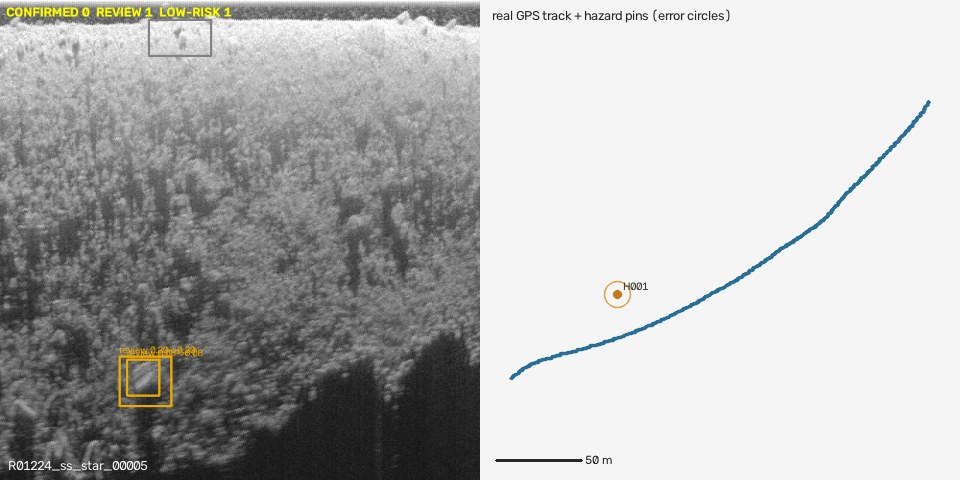
\includegraphics[width=\columnwidth]{figures/raw_recording.jpg}
\caption{\textbf{Raw Humminbird recording} (Colorado River, 150.6\,s, no known
pots). Left: one review card. Right: real GPS track and the resulting pin with
its 8.0\,m error circle.}
\label{fig:raw}
\end{figure}

\depth{} reads raw Humminbird files directly (Fig.~\ref{fig:raw}): 3{,}453 pings
per channel were parsed with no malformed records. GPS speed and the sonar's speed
field correlate at $r=0.95$, and course and heading differ by a median of
$2.4^{\circ}$. On the one-hour recording, the sounder cross-check resolved 280 of
280 chunks and corrected 3 of 3 gross tracking failures. The review load on water
without known pots is 24--48 cards per hour of sonar. Both recordings come from
another sonar, so the agent correctly withdraws its promise; these figures measure
false-alarm load, not recall.

% ------------------------------------------------------------ Negative res --
\section{Negative Results}

All studies were registered with their protocol before unseen data was scored.
We report the ideas that failed (Table~\ref{tab:neg}). The most instructive is
test-time augmentation: it added 0.10 AP on the recording used to select it and
lost 0.06 AP on unseen data, which only the fit-then-verify protocol revealed.

\begin{table}[t]
\centering\small
\setlength{\tabcolsep}{3pt}
\begin{tabular}{@{}p{3.35cm}p{4.35cm}@{}}
\toprule
Idea & Outcome \\
\midrule
Classical ROI gate & recall 0.708 $\rightarrow$ 0.147; retired \\
Shadow as a filter & precision 0.59 $\rightarrow$ 0.31--0.50; evidence only \\
Re-look re-scoring & no ranking gain; not used \\
Range-gain detector input & $\Delta$AP $-0.006$ [$-0.033$, $+0.019$] \\
Seam inference & no recall gain \\
Larger input + flip TTA & $+0.10$ AP calib., $-0.06$ AP unseen \\
Active vision (VoI tool choice) & both gates failed; off by default \\
EXP-002/004/005 recipes & did not beat EXP-003 \\
\bottomrule
\end{tabular}
\caption{\textbf{Negative results}, each from a registered study.}
\label{tab:neg}
\end{table}

% ------------------------------------------------------------- Limitations --
\section{Limitations}

\textbf{Detector accuracy.} mAP@0.5 is 0.319 against a 0.70 target, and the
crab-pot F1 trails the state of the art. \depth{} makes the detector usable, not
accurate. \textbf{Transfer.} A new sonar requires re-calibration; the
applicability test detects a different sensor but is not designed for gradual
drift in site or gain. \textbf{Guarantee scope.} The promise is a pooled rate
fitted on three recordings and verified on three; one recording fell below it.
\textbf{Field validation.} No recording has both labelled pots and real GPS, so
positions on pot frames use labelled synthetic tracks. \textbf{Human factors.}
Analyst times are assumed; the timed user study and blinded false-alarm audit are
built but not yet run, and incomplete labels make measured precision a lower
bound. \textbf{Failure modes.} On the earlier model, 32\% of missed pots touched
the frame edge (11\% of found pots), and misses had lower contrast and longer
range but were not smaller. \textbf{Sensing.} Pitch and roll are not corrected,
data dropouts are flagged rather than repaired, and outputs are boxes rather than
masks. \textbf{Deployment.} The COOL benchmark and edge hardware remain
unmeasured.

% -------------------------------------------------------------- Conclusion --
\section{Conclusion}

\depth{} shows that an imperfect sonar detector can support operational
decisions when it is wrapped in calibrated guarantees, an applicability test and
measured geometry. The agent promises, with 95\% confidence, that at least 78\% of
crab pots reach a person (84\% when looking harder); both promises held on unseen
recordings and survived a correction for correlated frames. It withdraws its
promise where it would be false, places findings where the measurements put them,
and acts only with human approval, all on a CPU with OpenCV~5. Because the
calibration code is model-agnostic, a stronger detector can be substituted and its
promise re-fitted with a single command.

\vspace{2pt}
\noindent\textbf{Acknowledgements.} We thank the GhostVision and PING-Mapper
authors for releasing their data. An AI coding assistant wrote much of the code
under the author's direction; every number in this paper is produced by a script
in the repository.

% -------------------------------------------------------------- References --
{\small
\begin{thebibliography}{99}\setlength{\itemsep}{0pt}
\bibitem{fao} FAO. Abandoned, lost or otherwise discarded fishing gear.
\url{https://www.fao.org/fishery/en/topic/16999}.
\bibitem{vims} VIMS Center for Coastal Resources Management. Marine Debris
Program. \url{https://www.vims.edu/ccrm/research/marine_debris/}.
\bibitem{russwurm2023} M.~Rußwurm, S.~J.~Venkatesa, and D.~Tuia. Large-scale
detection of marine debris in coastal areas with Sentinel-2. arXiv:2307.02465,
2023.
\bibitem{ghostvision} C.~S.~Bodine \etal{} GhostVision: Democratizing derelict
gear detection using low-cost sonar and artificial intelligence. \emph{J.\ Mar.\
Sci.\ Eng.}, 14(10):951, 2026.
\bibitem{pingmapper} C.~S.~Bodine, D.~Buscombe, R.~J.~Best, J.~A.~Redner, and
A.~J.~Kaeser. PING-Mapper: Open-source software for automated benthic imaging and
mapping using recreation-grade sonar. \emph{Earth and Space Science},
9:e2022EA002469, 2022.
\bibitem{yolo} J.~Redmon, S.~Divvala, R.~Girshick, and A.~Farhadi. You only look
once: Unified, real-time object detection. In \emph{CVPR}, 2016.
\bibitem{yolo11} G.~Jocher and J.~Qiu. Ultralytics YOLO11, 2024.
\url{https://github.com/ultralytics/ultralytics}.
\bibitem{onnx} ONNX: Open Neural Network Exchange. \url{https://onnx.ai}.
\bibitem{opencv} OpenCV. \url{https://opencv.org}.
\bibitem{clopper} C.~J.~Clopper and E.~S.~Pearson. The use of confidence or
fiducial limits illustrated in the case of the binomial. \emph{Biometrika},
26(4):404--413, 1934.
\bibitem{ltt} A.~N.~Angelopoulos, S.~Bates, E.~J.~Candès, M.~I.~Jordan, and
L.~Lei. Learn then test: Calibrating predictive algorithms to achieve risk
control. arXiv:2110.01052, 2021.
\bibitem{vovk} V.~Vovk, A.~Gammerman, and G.~Shafer. \emph{Algorithmic Learning
in a Random World}. Springer, 2005.
\bibitem{kunsch} H.~R.~Künsch. The jackknife and the bootstrap for general
stationary observations. \emph{Ann.\ Statist.}, 17(3):1217--1241, 1989.
\bibitem{voc} M.~Everingham, L.~Van~Gool, C.~K.~I.~Williams, J.~Winn, and
A.~Zisserman. The PASCAL visual object classes (VOC) challenge. \emph{IJCV},
88:303--338, 2010.
\bibitem{coco} T.-Y.~Lin \etal{} Microsoft COCO: Common objects in context. In
\emph{ECCV}, 2014.
\end{thebibliography}
}

\end{document}
